\documentclass{sigchi}

% Arabic page numbers for submission.  Remove this line to eliminate
% page numbers for the camera ready copy
% \pagenumbering{arabic}

% Load basic packages
\usepackage{balance}       % to better equalize the last page
\usepackage{graphics}      % for EPS, load graphicx instead 
\usepackage[T1]{fontenc}   % for umlauts and other diaeresis
\usepackage{txfonts}
\usepackage{mathptmx}
\usepackage[pdflang={en-US},pdftex]{hyperref}
\usepackage{color}
\usepackage{booktabs}
\usepackage{textcomp}
\usepackage{tikz}
\usetikzlibrary{positioning}
\usepackage{algorithm}
\usepackage{algorithmic}
\usepackage{caption}
\usepackage{tabularx}
\usepackage{array}
\usepackage{float}
% Some optional stuff you might like/need.
\usepackage{microtype}        % Improved Tracking and Kerning
% \usepackage[all]{hypcap}    % Fixes bug in hyperref caption linking
\usepackage{ccicons}          % Cite your images correctly!
% \usepackage[utf8]{inputenc} % for a UTF8 editor only

% If you want to use todo notes, marginpars etc. during creation of
% your draft document, you have to enable the "chi_draft" option for
% the document class. To do this, change the very first line to:
% "\documentclass[chi_draft]{sigchi}". You can then place todo notes
% by using the "\todo{...}"  command. Make sure to disable the draft
% option again before submitting your final document.
\usepackage{todonotes}

% Paper metadata (use plain text, for PDF inclusion and later
% re-using, if desired).  Use \emtpyauthor when submitting for review
% so you remain anonymous.
\def\plaintitle{Efficient Exctraction of True Random Numbers from Quantum System on Resource Constrained Hardware}
\def\plainauthor{First Author, Second Author, Third Author,
  Fourth Author, Fifth Author, Sixth Author}
\def\emptyauthor{}
\def\plainkeywords{Authors' choice; of terms; separated; by
  semicolons; include commas, within terms only; this section is required.}
\def\plaingeneralterms{Documentation, Standardization}

% llt: Define a global style for URLs, rather that the default one
\makeatletter
\def\url@leostyle{%
  \@ifundefined{selectfont}{
    \def\UrlFont{\sf}
  }{
    \def\UrlFont{\small\bf\ttfamily}
  }}
\makeatother
\urlstyle{leo}

% To make various LaTeX processors do the right thing with page size.
\def\pprw{8.5in}
\def\pprh{11in}
\special{papersize=\pprw,\pprh}
\setlength{\paperwidth}{\pprw}
\setlength{\paperheight}{\pprh}
\setlength{\pdfpagewidth}{\pprw}
\setlength{\pdfpageheight}{\pprh}

% Make sure hyperref comes last of your loaded packages, to give it a
% fighting chance of not being over-written, since its job is to
% redefine many LaTeX commands.
\definecolor{linkColor}{RGB}{6,125,233}
\hypersetup{%
  pdftitle={\plaintitle},
% Use \plainauthor for final version.
%  pdfauthor={\plainauthor},
  pdfauthor={\emptyauthor},
  pdfkeywords={\plainkeywords},
  pdfdisplaydoctitle=true, % For Accessibility
  bookmarksnumbered,
  pdfstartview={FitH},
  colorlinks,
  citecolor=black,
  filecolor=black,
  linkcolor=black,
  urlcolor=linkColor,
  breaklinks=true,
  hypertexnames=false
}

% create a shortcut to typeset table headings
% \newcommand\tabhead[1]{\small\textbf{#1}}

% End of preamble. Here it comes the document.
\begin{document}

\title{\plaintitle}

\numberofauthors{2}
\author{%
	\alignauthor{Love Arreborn\\
		\email{lovar063@student.liu.se}}\\
	\alignauthor{Nadim Lakrouz\\
		\email{nadla777@student.liu.se}}\\
}

\maketitle


\section{1 INTRODUCTION}\label{introduction}

In computer science, there are many applications for randomly generated numbers. From generating keys for cryptography, salting password hashes, load balancing in distributed systems, memory addressing and so much more. However, the process of producing these random numbers tends to be pseudo-random, e.g.~utilizing the current states of various modules \cite{randomness}. Pseudo-random numbers do not generate true randomness, and in order to heighten security, other methods of generating random numbers are required. Current random number generators (\emph{RNG}) are usually implemented in computer programs, using certain states of the host machine as a starting point before running a predetermined algorithm \cite{randomness}. This pseudo-random number generation (\emph{PRNG}) comes with the drawback that the result is always deterministic, provided that the initial state is known.

Imagine, then, if a malicious attacker somehow manages to ascertain the state a computer was in when it generated a random number, for instance to produce an SSH-key. This hypothetical attacker has the opportunity to accurately reproduce the exact, deterministic state that produced said random number, in essence removing the safety that randomness brings. While it may sound unrealistic, the exponential increase in processing power and the burgeoning field of quantum computing does introduce the possibility that one day, what we perceive as random is nothing more than a simple algorithm to crack.

True random numbers, then, cannot be produced solely through code. These systems require some input that is neither replicable nor reproducible. One method that can be realistically used is the inherently random movement of lava lamps \cite{lavarand}, which is used as a backup source of randomness for Cloudflare\footnote{\href{https://blog.cloudflare.com/randomness-101-lavarand-in-production/}{Cloudflare.com, accessed 2025-03-10}}. Another proposed solution for this is quantum random number generation (\emph{QRNG}) \cite{QRNG}. By reading quantum fluctuation signals from any given source, for instance an optical signal, the inherent natural unpredictability of said signal can be harnessed in order to produce a random number from a state that is nigh impossible to reproduce accurately. Clason \cite{Clason2023} presents a device that generates a fluctuating analogue signal utilizing this method.

The optical signal output by the device described in \cite{Clason2023} needs to be converted to a stream of random, raw bits via an Analog to Digital Converter (\emph{ADC}). Some post-processing of the said raw bits has to be performed in order to ensure that the bits are workable, and to remove potential deterministic patterns from the data. One method for this post-processing we will explore in this work is Toeplitz extraction \cite{toeplitz}, typically performed on the host computer utilizing the randomly generated numbers. The post-processing finally yields a random number. This relationship can be seen in Figure \ref{fig:linear-system}.

\begin{figure}[ht] \centering 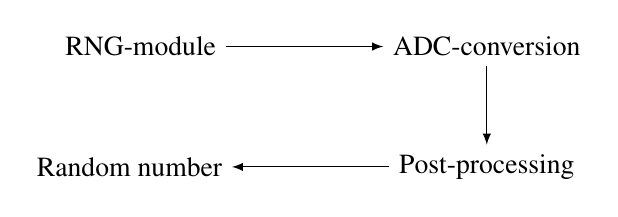
\begin{tikzpicture}[>=latex] % top row, 2 cm apart
\node (A) {RNG-module}; \node (B) [right=2cm of A] {ADC-conversion};

    \node (C) [below=1cm of B] {Post-processing};
    \node (D) [left=2cm of C]  {Random number};

    \draw[->] (A) -- (B);
    \draw[->] (B) -- (C);
    \draw[->] (C) -- (D);

\end{tikzpicture} \caption{An abstract of the steps required for OQRNG.}
\label{fig:linear-system} \end{figure}

Clason proposes a simpler and cheaper way to achieve QRNG \cite{Clason2023} than what has been done in previous research. These systems have generally been large, bulky and expensive, whereas the method proposed is portable enough to theoretically be installed in a portable device -- for instance a USB-thumbstick. In keeping with this, utilizing microcontrollers rather than a host computer for processing the raw bits extracted allows this system to be self-contained and portable, and further helps to keep the costs low and the solution reasonably complex.

However, due to the limited processing power of the average microcontroller, any implementation of Toeplitz extraction needs to work quickly and efficiently despite this hardware constraint. Experimenting with efficient implementations of this well-defined algorithm is the main focus of this thesis, and the key research areas explored in this work are as follows:

\textbf{Research area 1 (\emph{RA1})}: How can Toeplitz extraction be implemented as effectively as possible on resource constrained hardware in order to process raw bits into a workable random number?

Toeplitz extraction has been optimized quite well, and previous research can be utilized to address this research question. However, there are still considerations when implementing the firmware for the microcontroller in order to optimize the code. Our goal is to attempt several implementations in order to find the most optimal implementation with the least amount of effective processing time spent on the algorithm.

\textbf{Research area 2 (\emph{RA2})}: Can we ensure that the output of random numbers is not primarily limited primarily by our implementation, but rather limited by the processing power or the USB transfer speed of the microcontroller, alternatively by the ADC?

There will unequivocally be a bottleneck for the processing speed. For instance, the speed at which the ADC can process the optical signal into raw bits as well as the speed that the USB output can transfer processed random number to the host computer will be limiting factors. Further details on the limitations of the ADC will be outlined in Section 3. The slowest of these bottlenecks will inevitably be the limiting factor for any implementation. Our research aims to ensure that our implementation of Toeplitz extraction does not become the limiting factor, but rather processing data fast enough to match or exceed the speed of the hardware.

Section 2 of this article will introduce the theory that allows for QRNG, and how this will be utilized in our works. Section 3 delves further into the hardware and algorithms our work will use, with related works in optimizing Toeplitz extraction listed under section 4. Section 5 will present our methodology and implementation strategy, as well as some limitations imposed on our work. Finally, section 7 will present the results of our experimentation.

\subsection{2 THEORY}\label{theory}

A majority of the research around this topic stems from physics, with implementations of the technology frequently being published and studied by physicists. As such, a brief introduction to the concepts used in previous research as well as an introduction to previous implementations of this technology will be presented in this section.

The idea of an optical QRNG (\emph{OQRNG}) is not a novel one. The basis of the theory is the intrinsically random properties of a quantum process. Stefanov et. al. \cite{StefanovOptical} proposes using the random choice of a photon between two output signals to generate a random stream of bits, however the theory behind it can be applied to other quantum processes as well. This particular theorem has been implemented by Wayne et. al. \cite{Wayne} to create a quantum number generator. While this article proves the efficacy of OQRNG, it utilizes a slightly different method.

\subsubsection{2.1 Shot noise quantum fluctuations}\label{shot-noise-quantum-fluctuations}

Our work revolves around the measurement of shot noise of vacuum states rather than measuring arrival times of photons. Essentially, this is another quantum process with the same inherently random properties as described by Stefanov et. al. \cite{StefanovOptical}, but instead using shot noise. As described by Niemczuk \cite{shotnoise}, shot noise is minor fluctuations in an electrical current, which is inherently random. Reading this property, then, gives us an intrinsically random source from which to generate a random output, which in turn can be processed into a random number.

Implementations of this theory exist, however with significant drawbacks. Shen et. al. \cite{contender1} presents an implementation using a fairly complex setup, in which a continuous-wave fiber laser is the optical source. They conclude that sampling the shot noise is, indeed, suitable for OQRNG. However, the implementation requires expensive and complex hardware, and the sheer size of the system prohibits it from being portable and easily reproducible in small-scale tests.

A more recent implementation of OQRNG in a smaller scale has been presented by Singh et. al. \cite{singh}. This particular implementation uses a bespoke circuit board where all components are present on a single board -- e.g., this experimental setup contains an integrated ADC, post-processor, entropy controller and entropy generator. While this article cements the viability of OQRNG using shot noise (\emph{despite the article not being confirmed as peer reviewed}), the bespoke nature of the circuit board makes this experiment difficult to reproduce. As our thesis will use commercially available ADCs and microcontrollers, the only bespoke component is the shot noise generator itself. Furthermore, the Toeplitz extraction is not run on the microcontroller itself in these experiments -- instead, the hashing of these raw bits is done on the receiving computer as this bespoke circuit board featured a relatively weak processor.

In summary, previous research has proven that OQRNG can generate true randomness, and more specifically, Shen et. al. \cite{contender1} and Singh et. al. \cite{singh} both implement OQRNG through readings of shot noise. However, there are limitations in both of these works. Either the system that generates the shot noise is large and complex \cite{contender1} or the system is built on bespoke hardware with limitations in processing power which prevents a fully integrated system \cite{singh}. Furthermore, to the best of our knowledge, most of the work in this field is from the perspective of physicists, and there appears to be little research on this subject in the domain of computer science. Our work aims to bridge this gap by using commercially available hardware (\emph{other than the bespoke shot noise generator \cite{Clason2023}}) and focuses on implementing Toeplitz extraction directly on the microcontroller. Rather than focusing on the intricacies of quantum fluctuations, we will instead approach this problem from a computer science perspective.

\subsection{3 BACKGROUND}\label{background}

Our work is a practical continuation of the work of Clason \cite{Clason2023}. In this work, quantum shot noise originating from photodiodes was studied, and in so doing a prototype device was constructed. This prototype utilized an LED soldered millimeters apart from a photodiode, which in turn outputs a variable analog signal from the device. In this section, we introduce the remaining hardware used for our implementations as well as the considerations taken in order to shift the focus from physics to computer science.

\subsubsection{3.1 Optical RNG module}\label{optical-rng-module}

The one bespoke piece of hardware used in this study is the prototype designed by Clason \cite{Clason2023} as a part of his masters thesis. This device produces the optical shot noise which will be the source of randomness in our work. Moving forward in this article, we will refer to this as the OQRNG-device.

As described in Clasons work \cite{Clason2023}, the OQRNG-device is an electro-optical system which measures optical shot noise, generating quantum randomness. The device has an LED and a photodiode positioned a few millimeters apart, ensuring efficient light coupling. The photodiode detects light from the LED, and converts the light into a current signal, which is sent to a transimpedance amplifier to convert it into measurable voltage. In order to minimize disruptions by other external lights, the system is enclosed in a shielded measurment box.

Whereas the exact quantum mechanisms that ensure that this system ensures randomness and further details regarding the OQRNG-device is better derived directly from Clasons work \cite{Clason2023}, the primary concern for our study is the inherently random, analog voltage current produced by the system.

\subsubsection{3.2 ADC converter}\label{adc-converter}

This analog current is not suitable to operate on without further processing. As mentioned in Section 1, the signal needs to pass through an ADC to be converted into raw bits. In his thesis, Clason \cite{Clason2023} suggests a discrete ADC chip capable of analyzing frequencies higher than 25 MHz, as this is the highest frequency studied in his work. However, in the interest of keeping the implementation light and cheap, we will be using ADCs that provide less samples per second and lower frequencies. This is done mainly for ease of development and access to this hardware.

Many microcontrollers furthermore come equipped with internal ADCs that can be utilized, and while these provide a lower sample size (\emph{often around 1 MSPS}), the ease of development may be prudent to utilize for this proof-of-concept. While our initial ADC has a fairly low throughput, this can always be upgraded if it ends up becoming too limiting.

Should these internal ADCs prove too limiting, we propose utilizing MAX11102AUB\footnote{\href{https://www.farnell.com/datasheets/1913106.pdf}{Technical specification for MAX11102AUB, accessed 2025-03-13}} with an effective sample rate of 2 million samples per second (\emph{MSPS}). This ADC provides a 12 bit sample size, providing roughly 24 Mbit/s of sampled data per second, derived by the following calculation.

\[
\text{ADC Throughput}
= \frac{2,000,000_{\mathrm{MSPS}}\times12}{1,000,000}
\approx24\ \mathrm{Mbit/s}\phantom{123}(1)
\]

The final output from the ADC, whether built into the microcontroller or an external one, will be a stream of raw bits, as the analog signal from the OQRNG-device is processed.

\subsubsection{3.3 Microcontroller}\label{microcontroller}

Microcontrollers (\emph{MCUs}) are compact and low-power computing devices designed for embedded systems and real-time operations, and suitable as a processing unit for the purposes of this work. Unlike general CPUs, an MCU integrates a processor, memory and peripherals (\emph{such as an ADC}) into a single chip. Furthermore, modern MCUs often feature advanced microarchitectural elements to enhance processing capabilities on single threads (\emph{such as dual-issue superscalar architectures, allowing the MCU to run several instructions per CPU cycle}), making them suitable candidates for the post-processing required for OQRNG-data.

Since MCUs often function under strict timing requirements, it is critical to have effective ways to access memory and transfer data for processing in real time. High-performance MCUs enhance memory usage in various ways. Some of them use Tightly Coupled Memory\footnote{\href{https://www.farnell.com/datasheets/1913106.pdf}{Technical specification for MAX11102AUB, accessed 2025-03-13}} (\emph{TCM}), which gives fast SRAM with specific access routes for important data, avoiding cache misses and guaranteeing consistent performance. Moreover, instruction and data caching techniques, including instruction pre-fetching and branch prediction, help minimize execution delays in computationally intensive real-time applications. Another important aspect is Direct Memory Access\footnote{\href{https://www.sciencedirect.com/topics/computer-science/direct-memory-access}{ScienceDirect Journals \& Books, accessed 2025-03-13}} (DMA), which enables data transfer between peripherals such as the ADC and RAM, without CPU intervention. This offloading reduces processing overhead, allowing the MCU to manage fast data transfers effectively. These improvements are especially significant for Toeplitz extraction, where large amount of random data needs to be processed and sent quickly with low delays. Efficient memory management guarantees that randomness extraction can occur rapidly without major slowdowns in computing. Both approaches will be tested during development.

In our work, we intend to use Teensy 4.1\footnote{\href{https://www.pjrc.com/store/teensy41.html}{Teensy developer documentation, accessed 2025-02-27}}, based on the ARM Cortex-M7. This MCU is especially suitable for computationally demanding tasks involving randomness extraction due to its dual-issue superscalar architecture and Digital Signal Processing (\emph{DSP}) capabilities. The floating-point unit\footnote{\href{https://www.sciencedirect.com/topics/computer-science/floating-point-unit}{ScienceDirect Journals \& Books, accessed 2025-03-13}} (\emph{FPU}) and Single Instruction, Multiple Data (\emph{SIMD}) style DSP instructions improve how quickly it can perform bitwise and arithmetic tasks, which is crucial for quick Toeplitz extraction. SIMD-controlled DSP architectures, as described by Han et al. \cite{simd-dsp}, leverage parallel vectorized computation to accelerate matrix operations -- making them highly effective for Toeplitz matrix-vector multiplications.

In order to evaluate how efficent our implementation can become, our aim is to try our implementation on other MCU with different level of power and hardware support. Whereas Teensy 4.1, operating at \texttt{600\ MHz}, is our primary development platform which we will evaluate closely, we aim to run our implementations on the Raspberry Pi Pico 2\footnote{\href{https://datasheets.raspberrypi.com/pico/pico-2-product-brief.pdf}{Raspberry Pi Pico 2 documentation, accessed 2025-03-13}}, operating at \texttt{150\ MHz}. Due to the lower computational power of this MCU, there may be significant issues in utilizing this weaker model, yet it is significantly cheaper and easier to access. Testing will consist solely of running the implementation on these controllers and measuring execution speed and correctness of the output.

\subsubsection{3.4 Toeplitz extraction}\label{toeplitz-extraction}

The raw bits from the ADC can potentially have some deterministic patterns, and as such have to be processed somehow in order to remove these patterns. Several methods exist for this purpose, and for our work, we will perform this pre-processing via Toeplitz extraction. The main focus of this study is to implement this extraction algorithm as effectively as possible on resource constrained hardware.

A detailed account of the inner workings of Toeplitz extraction can be found in the work of Chouhan et al. \cite{toeplitz-desc}. This work focuses on implementing Toeplitz extraction on field-programmable gate-arrays (FPGA), but some specific details can be derived from their work. As these authors describe, Toeplitz extraction is a strong contender for our work due to a lower computational complexity than other alternatives, as well as a relatively easy algorithm to use. This extraction utilizes either matrix multiplication or hashing between a pseudo-random seed and the raw data provided from a high-entropy source of randomness -- in our case, the OQRNG-device.

To summarize the theoretical working of Toeplitz extraction (\emph{as explained by Chouhan et al. \cite{toeplitz-desc}}), a pre-determined seed matrix (\(T\)) is multiplied with the sampled raw bit matrix (\(K\)). The size of the seed is directly dependent on the size of the sampled data, and can be fixed or continually re-sampled as needed. To ensure high levels of entropy, our intuition is that re-sampling the seed from the OQRNG-device continually is prudent. The sample and seed will then be processed with matrix multiplication to remove deterministic patterns, and produce a bitstring that results in our randomly generated number. An example of how this extraction works can be seen below.

\begin{algorithm}[ht] \caption{Toeplitz extraction}\label{alg:bit-conv}
\begin{algorithmic}[1] \REQUIRE \(x[0\,..\,n-1]\) \Comment{input bit array of
length \(n\)} \REQUIRE \(t[0\,..\,n+m-2]\) \Comment{seed matrix of length
\(n+m-1\)} \ENSURE \(y[0\,..\,m-1]\) \Comment{output bit array of length \(m\)}
\FOR{\(i = 0\) to \(m - 1\)} \STATE sum = 0 \FOR{\(j = 0\) to \(n - 1\)} \STATE
sum = sum + \(x[j] \* t[i + j]\) \ENDFOR \STATE \(y[i] =
\mathrm{sum}\;\bmod\;2\) \ENDFOR \RETURN \(y\) \end{algorithmic} \end{algorithm}

The main focus of this work is implementing this algorithm as efficiently as possible on our MCUs, and as such, several optimization efforts need to be taken into account during our experimentation.

\subsubsection{3.5 Summary}\label{summary}

With the assumption that the OQRNG-device produces a truly random analog signal, we can now clearly define the scope in which this thesis operates. Considering the maximum conversion speed from the ADC and the USB-output from the MCU, we have a clear bound over 24 Mbit/s (\emph{imposed by the ADC}) in which Toeplitz extraction needs to be executed. Any speeds over 2.86 MB/s allows us to upgrade the ADC iteratively to continue increasing the output speed. Any implementation of Toeplitz extraction must then execute fast enough on any given microcontroller feasible for the proposed quantum RNG-thumbstick as to not be the decisive limiting factor.

\subsection{4 RELATED WORKS}\label{related-works}

Most related works found tend to revolve around optimizing Toeplitz using more advanced hardware, and few works seem to delve into evaluating the implementation in code.

As mentioned in section 3.4, Chouhan et al. \cite{toeplitz-desc} utilized FPGA to implement Toeplitz extraction specifically for OQRNG, a work also studied by Zhang et al. \cite{toeplitz}. Furthermore, Zhang et al.~utilized a standardized min-entropy evaluation to ensure true, unbiased randomness in their result. Both of these implementations utilize powerful hardware where the matrix multiplication is offloaded to FPGA. These implementations provided extraction speeds of between 3.36 Gpbs \cite{toeplitz} to 26.57 Gbps \cite{toeplitz-desc}. Neither of these implementations operate on constrained hardware, instead creating bespoke circuit boards for their works.

Another important point that is often neglected in randomness extraction using Toeplitz matrices is how the seed key is handled when forming the Toeplitz matrix. Numerous systems, such as those developed by Chouhan et al. \cite{toeplitz-desc} and Zhang et al. \cite{toeplitz}, depends on fixed seeds. Fixed seeds can create security risks over prolonged operation time. To tackle this problem, Lin et al \cite{lin} proposed a method for seed-renewable Toeplitz post-processing in QRNG. Their strategy incorporates a dynamic seed pool within the FPGA, where each instance of post-processing picks a new, randomly selected seed. Thus, minimizing temporal correlations between extractions. Furthermore, an external seed updating mechanism via Peripheral Component Interconnect Express (\emph{PCIe}) ensures that seeds are refreshed whenever a certain security limit is reached. Compared to fixed-seed methods, this renewable approach enhances cryptographic robustness and ensures sustained high-security randomness extraction in real-world applications.

Efficient Toeplitz matrix-vector multiplication (\emph{TMVM}) is critical for optimizing randomness extraction that relies on Toeplitz, particulary in constrained hardware environments. Liao et al. \cite{liao} showed that this process could be greatly accelerated using Fast Fourier Transform (\emph{FFT}) and its inverse (\emph{IFFT}) -- reducing computational complexity from \(O(n^2)\) to \(O(n \log n)\). Their implementation on FPGA utilized this approach for deep neural networks, resulting in a 28.7 times decrease in model size while still achieving fast inference speeds. By using FFT and IFFT acceleration, Toeplitz post-processing for randomness extraction could achieve higher throughput. Thus, potentially could improve performance and reduce latency.

\subsection{5 METHODOLOGY}\label{methodology}

With the consideration that our work revolves around optimizing Toeplitz extraction in order to quickly process random bits into a random number, we will take an iterative approach. For our tests, we will use a pre-defined stream of raw bits which is sent to the microcontroller via USB, and run several different implementations of Toeplitz extraction to produce numbers. As we always use a pre-defined bitstream, the result will at this stage be deterministic, giving us a clear indication whether the algorithm works as intended.

However, in order to ensure the results work with varying data, we cannot limit ourselves to simply one stream of bits. The main point of the algorithm is to remove patterns in the bitstream that may lead to less randomized results. As such, we will sample several bitstreams from the OQRNG-device to use for our tests -- each with varying degrees of repeated patterns that should be eliminated by the algorithm. All bitstrings tested are available as an appendix to this paper.

Our implementation of the Toeplitz extractor followed a structured, iterative approach divided into two phases. Phase one focused on exploring performance improvements through incremental algorithmic changes. Phase two then addressed architectural inefficiencies identified during phase one. Each phase then consisted of a number of individual iterations, in which performance was evaluated in terms of both correctness and execution time on the target hardware.

\subsubsection{5.1 Phase one}\label{phase-one}

Initially, we require a ``naive'' version designed to prioritize correctness over speed. This version was first executed on a separate computer to generate reference output for various input bitstrings, which were later used as accuracy baselines. The naive implementation was then flashed onto the Teensy 4.1 microcontroller, where execution time was measured in microseconds. Each subsequent iteration introduced controlled modifications aimed at improving throughput.

The initial implementation followed the pseudocode described in Algorithm \ref{alg:bit-conv}, using matrix multiplication over raw input and seed data. It relied on \texttt{std::vector\textless{}int\textgreater{}} for storage and used nested loops to compute each output bit. From this point, this implementation was improved over the coming iterations, and the new implementation verified in the same manner as the initial version.

\textbf{Iteration 1 - Data structures:} This iteration kept the same algorithmic logic as the initial implementation, but experimented with data structures such as raw pointers and hash maps to enhance the use of \texttt{std::vector}. The goal was to reduce or eliminate the reliance on nested loops.

\textbf{Iteration 2 - Bitshifting:} Basic bitwise operation was introduced to replace arithmetic whenever possible. Multiplication was replaced with logical \texttt{AND\ \&} and modulo operations with bit masking \texttt{\&\ 1}. The goal was to reduce the number of instructions and improve per-bit processing speed.

\textbf{Iteration 3 - Batching and Hardware optimization:} This iteration focused on optimizing performance through batching and the use of ARM-native instructions, beginning by testing batching alone. This was followed by isolated use of ARM instructions such as \texttt{\_\_builtin\_popcountll()} (\emph{which counts the number of set bits in an unsigned integer}). After establishing their individual effect we combined both techniques, multiple batch sizes were tested to determine their impact. More details and benchmarks for each configuration can be found in the section 6.

\subsubsection{5.2 Phase two}\label{phase-two}

Phase two focused on addressing inefficiencies and design issues that were unintentionally introduced during earlier iterations. Rather than continuing with new algorithmic ideas, this phase aimed to identify and fix structural problems. Several assumptions from phase one were re-evaluated -- such as the benefits of certain data structures or abstractions.

\textbf{Iteration 4 - Loop unrolling:} This iteration focused on reducing the number of loops in the extractor by manually unrolling repeated operations. The goal was to decrease overhead created by loops. Whereas this operation is commonly done by compiler optimization, manually performing this guarantees that we unroll the loops rather than leaving it to the compiler.

\textbf{Iteration 5 - Removal of vector usage:} This iteration removed \texttt{std::vector} in favor of fixed-size types like \texttt{uint32\_t} and \texttt{uint64\_t} to reduce the overhead introduced by creating and populating this complex data structure.

\textbf{Iteration 6 - Data type exploration:} Following the removal of vectors, this iteration explored alternative static data types such as: \texttt{array}, \texttt{unordered\_map} and \texttt{bitset} to determine the most efficient structure for storing input and seed data.

\subsubsection{5.3 Evaluation}\label{evaluation}

To evaluate the correctness of each implementation, a baseline was generated as discussed in section 5.2. Using the naive, initial implementation to process bits and saving for later evaluation gave us a source of truth against which to compare following iterations. To verify that the algorithm successfully removed the patterns it should, we verified the measured entropy score with the command line utility \texttt{ent}\footnote{\href{https://manpages.ubuntu.com/manpages/trusty/man1/ent.1.html}{Manual page for \texttt{ent}, accessed 2025-04-23.}}. This tool verifies the statistical randomness of any given file, and does several calculations to provide an estimate of how random any given binary file is.

The way \texttt{ent} calculates the entropy of a given binary file is by checking the frequency of certain byte values. If some byte values are more frequent, the binary file has a low entropy -- essentially singifying that there are predictable patterns. Conversely, if all byte values appear roughly equally, the binary file has a high entropy -- meaning that it is more random, and less predictable. The maximum entropy of any given file is \(\log_2(256) = 8 \text{ bits per byte}\), meaning that a perfectly random binary file has an entropy score of 8. For the purposes of our work, we consider values greater than \(7.99\) to be acceptable.

Furthermore, \texttt{ent} also provides a measurement of the possible compression ratio of the file, e.g.~how much more the file can be theoretically compressed. This is calculated as \(1 - \frac{\text{entropy}}{\text{maximum entropy}}\), signifying that the file cannot be compressed further -- that the data is already as compressed as its random distribution allows. Essentially, this informs us that the file has no more detectable statistical patterns or compressable regularities remaining. We consider any file where \texttt{ent} reports a compression ratio of \(0\%\) to be acceptable.

Hyncica et. al. \cite{micromeasurements} propose that measuring execution time of algorithms directly via the microcontrollers internal timers (while subtracting the interrupt overhead) provides adequate measurements of the execution speed of an algorithm. An additional advantage is that the same code can be used to measure execution speed on several different microcontrollers, rather than relying on counting CPU cycles (as the process for this may vary greatly between controllers).

In our implementation, execution time for each extraction was measured using Arduino's built-in \texttt{micros()}\footnote{\href{https://docs.arduino.cc/language-reference/en/functions/time/micros/}{Documentation for \texttt{micros()}, accessed 2025-05-02.}} function. This function offers a convenient and platform-independent method for recording elapsed time with microsecond precision, enabling consistent performance evaluation across different iterations.

As we will use fixed-size bitstrings for evaluation, we can then derive the throughput of the algorithm in \(Mbit/s\) as follows:

\[
Throughput_\mathrm{Mbit/s}
= \frac{DataSize_\mathrm{bits}}{ExecutionTime_\mathrm{ms}}
\times 10^{-3}
\phantom{12}(2)
\]

This measurement allows us to place the throughput of our algorithm soundly in the bounds imposed on us by the hardware. Plugging in the \(24 Mbit/s\) bound imposed by the ADC with an arbitrarily chosen 64-bit sample size, we can derive the average execution speed in microseconds:

\[
\frac{64}{24}\times10^{-3}\ \mathrm{ms}
\approx 2.667\times10^{-3}\ \mathrm{ms}
=2.667\ \mu\mathrm{s}.
\phantom{12}(3)
\]

In section 6, this calculation will be used to derive the execution speed of the various iterations.

\subsubsection{5.4 Limitations}\label{limitations}

Our proposed iterations all assume that the limited hardware will support it. Whereas we are confident that Teensy 4.1 will be able to handle each iteration step (\emph{even the naive implementation}), the remaining microcontrollers with lower specifications might not be suitable for the first iterations. Testing the implementations on different microcontrollers could turn out to be unfeasible -- however, this remains to be seen during the experimentation.

\subsection{6 RESULTS}\label{results}

We created a script to facilitate easier testing, which is attached to this paper. Using this script, all bitstrings used for testing can be evaluated against the baseline, ensuring that the output from the new iteration matches the baseline exactly. Furthermore, the script also provides the average execution time of only the Toeplitz extraction in microseconds. A brief overview of the architecture of this test script can be seen in Figure \ref{fig:testscript-architecture}.

\begin{figure*}[!t] \centering
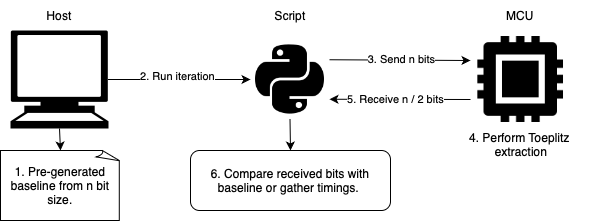
\includegraphics[width=\textwidth]{img/testscript.png} \caption{A brief overview
of the testscript architecture.} \label{fig:testscript-architecture}
\end{figure*}

\subsubsection{6.1 Phase one}\label{phase-one-1}

\vspace{1em}

\begin{table}[ht] \centring
\begin{tabularx}{\columnwidth}{|>{\centering\arraybackslash}X|>{\centering\arraybackslash}X|>{\centering\arraybackslash}X|}
\hline \textbf{Bit size} & \textbf{Teensy ($\mu$s)} & \textbf{Pico ($\mu$s)} \\
\hline 64 & 13.1564 & 106.3914 \\ 512 & 788.3139 & 5302.4979 \\ 1024 & 3124.0580
& 21111.2163 \\ \hline \end{tabularx} \caption{Iteration 1 - Data Structures}
\label{tab:iter1} \end{table}

Table \ref{tab:iter1} presents the average execution time of iteration 1 on both Teensy 4.1 and Raspberry Pico Pi 2 across the input sizes. The Teensy consistently outperforms the Pico, with the gap widening as the bit size increases.

\begin{table}[ht] \centring
\begin{tabularx}{\columnwidth}{|>{\centering\arraybackslash}X|>{\centering\arraybackslash}X|}
\hline \textbf{Bit size} & \multicolumn{1}{c|}{\textbf{Teensy ($\mu s$)}} \\
\hline 64 & 16.4689 \\ 512 & 1006.6255 \\ 1024 & 3996.5972 \\ \hline
\end{tabularx} \caption{Iteration 2 - Bitshifting} \label{tab:iter2} \end{table}

Table \ref{tab:iter2} shows the execution times for iteration 2 on the Teensy 4.1, which utilizes bitshifting instead of the original data structure approach. A clear increase in executiom time compared to iteration 1 is observed.

Additionally, the isolated effect of applying a single bitmask operation \texttt{\&\ 1} was evaluated. This resulted in a slight reduction in average execution time, from \texttt{13.1564} \(\mu s\) to \texttt{13.1000} \(\mu s\), although this specific result is not included in the tables above.

\begin{table}[H] \centring
\begin{tabularx}{\columnwidth}{|>{\centering\arraybackslash}X|>{\centering\arraybackslash}X|}
\hline \textbf{Bit size} & \multicolumn{1}{c|}{\textbf{Teensy ($\mu s$)}} \\
\hline 64/64 & 43.0760 \\ 512/512 & 2663.8194 \\ 1024/1024 & 10513.1767 \\
\hline \end{tabularx} \caption{Iteration 3 - Batching and Hardware optimization}
\label{tab:iter3} \end{table}

Table \ref{tab:iter3} presents the average execution time of iteration 3 on the Teensy 4.1 for varying batching and bit sizes. Additionally, when performing the same 1024/1024-bit operation, the Raspberry Pi Pico 2 showed average execution time of \texttt{80806.006} \(\mu s\) indicating a substantially lower throughput compared to the Teensy.

\subsubsection{6.2 Phase two}\label{phase-two-1}

\vspace{1em}

\begin{table}[ht] \centring
\begin{tabularx}{\columnwidth}{|>{\centering\arraybackslash}X|>{\centering\arraybackslash}X|>{\centering\arraybackslash}X|}
\hline \textbf{Bit size} & \multicolumn{1}{c|}{\textbf{Teensy ($\mu s$)}} &
\multicolumn{1}{c|}{\textbf{Pico ($\mu s$)}} \\ \hline 64 & 9.7017 & 70.7402 \\
512 & 551.6358 & 3978.1928 \\ 1024 & 2195.1979 & 15830.8784 \\ \hline
\end{tabularx} \caption{Iteration 4 - Loop unrolling} \label{tab:iter4}
\end{table}

Table \ref{tab:iter4} presents the execution time of iteration 4, which utilizes a 4x unrolled bit-processing loop. Compared to erlier iterations, this approach yields a substantial performance improvments on both the Teensy and the Raspberry Pi Pico Mcu's.

In addition to the results presented in Table \ref{tab:iter4}, a further tests was conducted on the Teensy using a single-loop unrolled implementation for the 64-bit size, resulting in an average execution time of \texttt{6.6626} \(\mu s\). An additional fully unrolled variant, where loops were entirely eliminated, produced a measured execution time of \texttt{0.0491} \(\mu s\). However, this measurement was later determined to be invalid due to packaging error.

\vspace{1em}

\begin{table}[ht] \centring
\begin{tabularx}{\columnwidth}{|>{\centering\arraybackslash}X|>{\centering\arraybackslash}X|>{\centering\arraybackslash}X|}
\hline \textbf{Bit size} & \multicolumn{1}{c|}{\textbf{Teensy ($\mu s$)}} &
\multicolumn{1}{c|}{\textbf{Pico ($\mu s$)}} \\ \hline 64 & 0.0501 & 0.2175 \\
\hline \end{tabularx} \caption{Iteration 5 - Removal of vector usage}
\label{tab:iter5} \end{table}

Table \ref{tab:iter5} presents the results of iteration 5, in which vector structure were removed in favor of fixed-size integer types \texttt{uint32\_t} and \texttt{uint64\_t}. This iteration led to an extremely efficient implementation that approaches the physical execution limits of the Teensy 4.1.

\vspace{1em}

\begin{table}[H] \centring
\begin{tabularx}{\columnwidth}{|>{\centering\arraybackslash}X|>{\centering\arraybackslash}X|}
\hline \textbf{Data structure} & \multicolumn{1}{c|}{\textbf{Teensy ($\mu s$)}}
\\ \hline array & 0.4284 \\ unordered_map & 31.5090 \\ bitset & 0.0474 \\ \hline
\end{tabularx} \caption{Iteration 6 - Data type exploration} \label{tab:iter6}
\end{table}

Table \ref{tab:iter6} presents the results of iteration 6 using 64 bit size, which was introduced to address the structural limitations encountered in iteration 5. Specifically, the fixed-width output constrains imposed by the removal of vector. In this iteration, alternative data structures were evaluated. Vector-based approach from iteration 1 serving as a baseline for comparison.

Additionally, 128 bit size were tested resulting in \texttt{179.8712} \(\mu s\).

\subsection{7 DISCUSSION}\label{discussion}

Observing the results, we can place them into the context of the limits imposed by the ADC, as discussed in Section 3.2. In algorithm (3) (\emph{as seen in Section 3.3}), we calculate the average execution speed required to be \(2.667 \mu\) for the ADC that requires soldering to the microcontroller. From Tables \ref{tab:iter5} and \ref{tab:iter6} we demonstrate execution speeds well below that, with iteration 5 as well as iteration 6 -- specifically with bitsets -- being the most prominent results to discuss. Here, our implementation achieved speeds of \(0.0501 \mu s\) and \(0.0474 \mu\) respectively which within the bounds of the ADC listed in Section 3.2. The built in ADC on Teensy has an effective sample rate of 1 MSPS (\emph{e.g.~half of MAX11102AUB}), which would require an average execution speed of \textasciitilde{}\(2.667/2 \mu s \approx 1.334 \mu s\), making our implementation suitable even for that limited conversion speed.

The main culprit that led other iterations to not be viable was the inclusion of \texttt{std::vector}, which was used to ensure we could deliver variable lengths of our return data -- e.g.~either 32, 64 or 128 bits. The overhead introduced from initializing and populating the vector led to significant delays in execution speed, leading to all other attempts at optimization to be superfluous. In fact, any other complexities led to significantly worse results than the naive, original implementation.

However, it is important to note that both of these implementations has a hard limit of working on 64 bits input. Whereas larger bitstrings still yield results with high entropy, the execution speed increases far above the hardware limitations, as evident in \ref{tab:iter6}. Iteration 5 is hard capped at using only 64 bits input, as we need to store the bits in fixed-size integers before running them through the algorithm, and on embedded machines we have no larger integer types available.

One issue still remains concerning the size of the input string and subsequent output string. The larger the size of the matrix provided to the Toeplitz function (\emph{e.g.~the larger our input}), the higher the potential overall entropy becomes. As our implementation is essentially capped at 64 bits input at this point in time (\emph{without being limited by the hardware}), this may or may not prove to not be secure enough for use in real world applications. This, however, is out of scope for this particular thesis, but a consideration nonetheless.

Any requirement of output integers larger than 32 bits may prove problematic. Whereas the bits processed by the algorithm does show an entropy measure quite close to 8, e.g.~reliably random, this does not necessarily mean that two sets of 32 bits can be combined on the host machine to produce a 64-bit integer. Combining these two sets may very well result in a less random result -- in essence, an entropy score that is not entirely random. As quantum computing evolves, the process of bruteforcing algorithms with all possible numbers becomes less of an impossible task, which is why this process of generating random numbers is required. The purpose of using quantum flucuation for random number generation is to provide greater assurances of security not possible from traditional, pseudo-random RNG, and being so severely limited by the size of the output is a major flaw in this implementation worth considering.

\subsection{8 CONCLUSION}\label{conclusion}

This work set out to investigate the feasibility of implementing Toeplitz extraction on resource constrained hardware. Furthermore, we aimed to conclude whether the extraction algorithm could be executed fast enough to not be the limiting factor, e.g.~that the speed of the extraction did not exceed the speed of the ADC conversion. Ostensibly, these investigations were both successful, considering that we managed to create an implementation that executes in roughly one half microsecond on average, far exceeding the limits imposed by the ADC. The optimization with the algorithm revolved around removing as much complexity as possible, avoiding anything that is not the simplest form of data structure for maximum performance gains.

As mentioned in Section 7, this comes at a price. The implementation that did indeed perform above expectation could only output a 32-bit integer, as we cannot take any larger input than 64 bits without any more complex data structure. How much of a flaw this is for a system utilizing this method of OQRNG is beyond the scope of this thesis to investigate. However, it is likely that a larger output is required for any application revolving around tight security. For less critical systems and less essential functionality, this method might, however, prove just secure enough. For instance, an IoT-device that requires a random number output for symmetric cryptography when connecting to a user device may be an ideal candidate for this method of OQRNG.

\subsection{9 FUTURE WORK}\label{future-work}

The main limitation for producing output with a larger size is the lack of a suitable data type in the limited standard library available for MCUs. Furthermore, it appears as if generic containers (\emph{such as \texttt{std::vector}}) that have already been severely optimized still impose a far greater performance penalty for this purpose. Future work may focus on implementing custom data types for larger bit sizes, for instance 128-bit and 256-bit integers. It may be possible that external libraries exist that alredy provide implementations of these integer sizes, but even then a slimmed down and customized implementation may prove the better alternative for this extreme performance constraint.
% BALANCE COLUMNS
\balance{}

% REFERENCES FORMAT
% References must be the same font size as other body text.
\bibliographystyle{SIGCHI-Reference-Format}
\bibliography{sample}

\end{document}

%%% Local Variables:
%%% mode: latex
%%% TeX-master: t
%%% End:
